\documentclass{report}

% Language setting
% Replace `english' with e.g. `spanish' to change the document language
\usepackage[english]{babel}
\usepackage{blindtext}
\usepackage{titlesec}

% Set page size and margins
% Replace `letterpaper' with `a4paper' for UK/EU standard size
\usepackage[a4paper,top=2cm,bottom=2cm,left=3cm,right=3cm,marginparwidth=1.75cm]{geometry}

% Useful packages
\usepackage{amsmath}
\usepackage{float}
\usepackage{caption}
\usepackage[skip=0.5ex]{subcaption}
\usepackage{graphicx}
\usepackage{xcolor}
\usepackage[
colorlinks=true,urlcolor=blue,linkcolor=purple,citecolor=red
]{hyperref}
\usepackage[toc]{appendix}
\usepackage{markdown}

\usepackage[table,xcdraw]{xcolor}
\usepackage{adjustbox}
\usepackage{url}


\usepackage{csquotes}
\usepackage[
backend=biber,
style=ieee,
]{biblatex}
\addbibresource{sources.bib}

%\usepackage[Conny]{fncychap}
%\ChNameAsIs
%\ChTitleAsIs
\pagestyle{headings}

\title{Enabling photodetection electronics for 
	fluorescent diamond based quantum sensing \\Project plan}
\author{Vladislav Serafimov}

\begin{document}
	\maketitle
	
	\tableofcontents
	
	\chapter{Introduction}
	This chapter introduces the assignment and some foundational concepts of quantum sensing.
	
	\section{Background}
	Nitrogen-vacancy (NV) centers \cite{enwiki:1301369588} are imperfections in the atomic structure of diamonds, which have the useful property of spin-dependent luminescence. This means that the spin of the NV center affects the frequency of the light emitted by the structure\footnote{The NV center only emits light after absorbing photons, a phenomenon called photoluminescence \cite{enwiki:1309081879}}. Using this quality of the NV structure, different environmental metrics (e.g magnetic fields) can be measured. 
	
	The Applied Nanotechnology research group is working on a NV-center-based sensor setup. Processing data from the setup requires working with weak signals that are hard to distinguish from the environmental noise. While this is a significant problem, it is also a very common one. Because of this, there is already widely-used system used to isolate signals in such cases: the lock-in amplifier.
	
	\section{Purpose of the assignment}\label{purpose}
	Implementing a lock-in amplifier is the main purpose of the assignment. To create a complete solution, there are several different functionalities and systems that need to be developed. 
	
	Before doing anything else, the raw sensor data needs to be extracted and then fed to a lock-in amplifier. This should be done in a standardized manner, in order to facilitate testing with different devices. After establishing connection, a control interface needs to be implemented. It needs to be programmed so that it can control all necessary features of the lock-in amplifier. Following the development of the program, a custom photodetection circuit needs to be designed. The circuit should accommodate the sensors and lock-in amplifier. Lastly, an OLIA\footnote{Open Lock-In Amplifier (OLIA) is an open-source microcontroller-based lock-in amplifier. It uses common components, which makes it easy to build \cite{harvie2023olia}} circuit needs to be tested and compared to conventional lock-in systems. 
	
	
	\section{Assignment specifications}\label{specifications}
	As already explained, the assignment is quite broad and involves both hardware and software, causing the need for a number of different tools. 
	
	Most of the hardware tools are already available at the Applied Nanotechnology lab. The lock-in amplifiers which will be used for the tests are the most important pieces of hardware. Zurich Instruments HF2LI is the benchmark lock-in amplifier. There are several different photodetectors available and the one which fits the project best will be picked at a later date. 
	
	In terms of software, there is more freedom of choice. Interfacing with the ZI HF2LI is done through proprietary software, but this is the only required program. There are various electronic computer-aided design (ECAD) software suites that offer the same base functionality. KiCad was selected because the client prefers open-source software. The program for retrieving data from the lock-in amplifiers can be written in both Python and MATLAB. Both languages have good integration with the main lock-in amplifier. They also offer graphic user interface (GUI) programming capabilities and are good for scientific computing overall.
	
	%Figure \ref{openremote_diagram} shows a diagram of all the functionalities offered by OpenRemote. In brief, OpenRemote is a platform for managing IoT devices. The most important features for this project are the MQTT agents (functioning as brokers/clients) and the built-in data visualization options. 
	
	
	%The languages used for this project will be Python and C/C++. The extensive and varied catalog of Python packages makes the language better for tasks where simplicity is valued over speed. Because of this, during the project, Pyhton will be used for modeling and visualization of the data. The MQTT communication can be done using both, which means they need to be evaluated during the project to see which one suits it better.
	
	%Data visualization and modeling will both be done, at least partially, in Python. `matplotlib` is one of the most widely-used packages for data visualization and because of this it was chosen for this project as well. Because OpenRemote has built in features for data plotting, it will also be used for some visuals. Data modeling, using statistical models, will be done in order to make sure the final product is configured in the optimal way. The optimal configuration will balance performance and service availability. Python's relevant features are the reason it was chosen for this task as well. 
	
	%The extra features will use the same languages. C/C++ is more suited to low-level applications, so it will be used for the firmware. Python has a plethora of features and packages that make it good specifically for machine learning, so data prediction will be done in Python.
	
	
	\section{Methodological approach}\label{methodological_approach}
	The V-Model methodology was selected, as it is well-suited for low-level projects. Figure \ref{fig:vmodel} shows a diagram of the phases of the V-Model. Unlike some software-oriented models, the V-Model is very sequential. This can sometimes be seen as detrimental, but in this case it helps with structuring the project. Another benefit of this model is that there are multiple testing activities, which underpin the quality assurance. A contentious feature of the V-Model is the heavy reliance on the initial requirements. This need for deliberate project requirements can be hard to meet, especially if the client representative is not technically proficient. However, this is not the case in this project. The requirements were extensively discussed with the client representative, based on which the project boundaries in Chapter \ref{project_boundaries} were set up.
	
	\begin{figure}[ht]
		\centering
		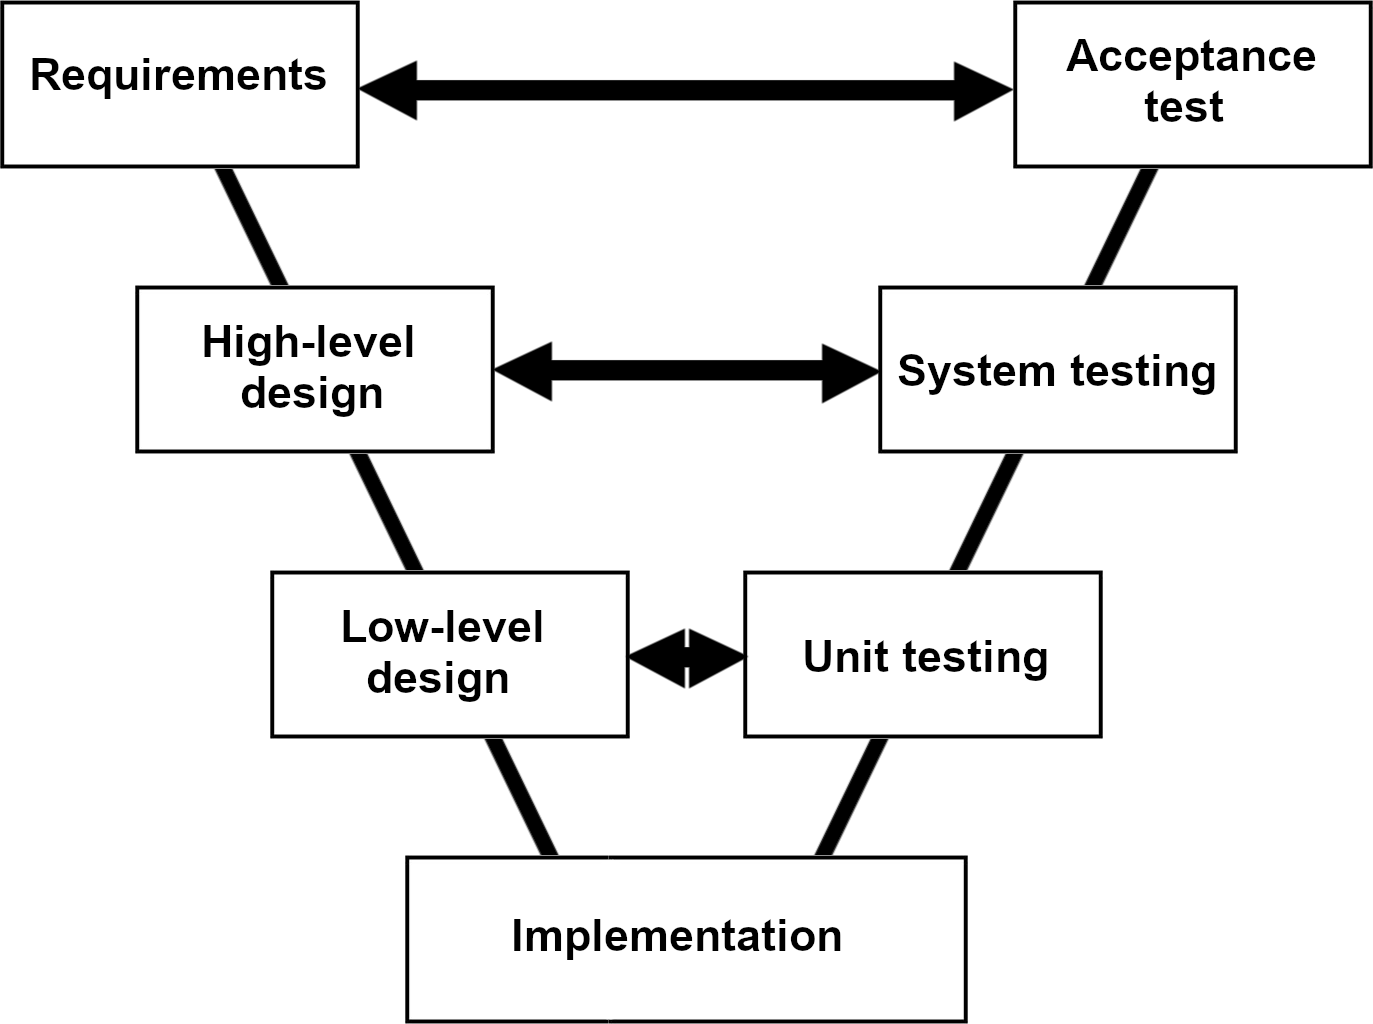
\includegraphics[width=0.7\linewidth]{img/vmodel}
		\caption{V-Model diagram}
		\label{fig:vmodel}
	\end{figure}

	\chapter{Project boundaries} \label{project_boundaries}
	The project boundaries were initially based on the assignment form, but were later discussed with the client and refined further. 
	
	\textbf{Must have}
	\begin{itemize}
		\item Hardware platform for photodetection
		\item Software for signal processing and visualization
	\end{itemize}
	
	\textbf{Should have}
	\begin{itemize}
		\item Tests with different diamond samples
	\end{itemize}
	
	\textbf{Could have}
	\begin{itemize}
		\item Tests with different quantum protocols
		\item OLIA implementation
		\item Tests comparing OLIA to market solutions
	\end{itemize}
	
	\textbf{Will not have}
	\begin{itemize}
		\item 
	\end{itemize}
	
	
	\chapter{Products and project objectives}
	This chapter describes all the required products and based on them sets up the objectives for the project.
	
	\section{Products}
	There are several technical products that need to be delivered, all of which fall into the categories of hardware, software and test data.
	
	Developing a hardware platform for measurements is the most important part of the project. The photodiode subsystem needs to be in the form of a printed circuit board (PCB). It needs to have output connectors that can accommodate a lock-in amplifier. Additionally, an OLIA can also be built using the available schematics. 
	
	In terms of software, an application needs to be developed to process and visualize the signal readouts from a lock-in amplifier. It should be able to retrieve data from different lock-in amplifiers. If necessary, modifications to the OLIA firmware will also be made. 
	
	Lastly, performance measurements also need to be delivered to the client in a digestible manner. Test data should compare performance of different lock-in amplifiers using different diamond samples. The most important metrics are signal-to-noise ration (SNR), bandwidth and stability. If there is enough time at the end of the project, tests with alternative quantum protocols can be done. Finally, if an OLIA was built, it needs to be compared in the same way to the different lock-in systems available on the market.
	
	\subsection{Goals} \label{chap:goals}
	% goals are tasks now, change to goals
	Based on the MoSCoW priorities from Chapter \ref{project_boundaries}, a set of goals was created to further specify all items from each prioritization category. Every goal was designed so that its outcome results in a tangible project milestone (e.g. a deliverable).
	
	\begin{itemize}
		\item[Goal 1]: Create a hardware setup, which measures and amplifies photodiode signals
		\item[Goal 2]: Develop software to process and visualize lock-in amplifier signals
		\item[Goal 3]: Compare the performance of different lock-in amplifiers
	\end{itemize}
	
	While these goals are practical, they are still not specific enough. To eliminate the possibility of confusion, a set of tasks were created. All tasks contribute to one of the three goals.
	
	\begin{itemize}
		\item[Task 1.1]: Design a photodiode PCB, which can accommodate different lock-in amplifiers
		\item[Task 1.2]: Build an operable OLIA
		\item[Task 2.1]: Develop software that acquires signals and is then able to visualize them
		% TODO: ask about task 2.2
		%\item \textbf{Task 2.2}: Apply digital signal processing techniques to signals acquired by the software 
		\item[Task 3.1]: Use key performance metrics to compare the OLIA implementation to market solutions
		\item[Task 3.2]: Measure OLIA performance using different diamond samples and quantum protocols
	\end{itemize}
	
	\textbf{Task 1.1} involves the design and production of a photodiode PCB. The PCB has to output signals that are not only compatible with lock-in amplifiers that are available on the market, but also with the OLIA. This part of the hardware design has the highest priority, which is why it will be done first. 
	
	\textbf{Task 1.2} is to build an OLIA amplifier, which can be used at Applied Nanotechnology's laboratory. This will be done with the technical specifications and firmware provided by Harvie and de Mello \cite{harvie2023olia}. The necessity for an OLIA is low, because the Applied Nanotechnology research group already has two lock-in amplifiers.
	
	\textbf{Task 2.1} is to write an application in Python or MATLAB. This can be done on a different setup, but ideally it will use the hardware setup from \textbf{goal 1}. Because the OLIA project uses open-source firmware that differs from proprietary solutions, there might need to be two separate applications. This task can only be completed once a measurement setup is built, so its execution will follow the first two tasks.
	
	%\textbf{Task 2.2} 
	
	\textbf{Task 3.1} requires all previous tasks to be finished. The completed setup needs to be used to measure the performance of lock-in amplifiers available on the market and the OLIA implementation. SNR, bandwidth and stability are the main metrics that need to be compared.
	
	\textbf{Task 3.2} is similar to \textbf{task 3.1}, but it is a much broader exploration of the performance of the lock-in amplifiers. Using different diamond samples and quantum protocols will show how the amplifier performs and how different conditions affect it. Because the task can be used to verify the setup from \textbf{goal 1}, it can also be done before \textbf{task 3.1}. Tests with varying diamond samples are more important to the client, which is why they will take precedence over tests with different quantum protocols.
	
	
	\subsection{Deliverables}
	The description of the tasks already provided context for the deliverables, but this subsection contains a formalized version of the deliverables.
	
	\begin{enumerate}
		\item Photodetection PCB 
		\item OLIA
		\item Software application
		\item Comparison visualization
		\item Technical documentation
	\end{enumerate}
	
	The only deliverable, which was not mentioned in Chapter \ref{chap:goals} is the technical documentation. This is because it should contain information about every task.
		
	
	\chapter{Project activities}
	Based on the V-Model from Chapter \ref{methodological_approach}, four types of activities can be established: requirements, design, implementation and testing. Additionally, documentation is also an activity that is integral to the project.
	
	\section{Requirements}
	As already discussed, establishing requirements should be done deliberately, so that no changes need to be made during the project. Several different activities are needed for this stage of the project. One of the most productive ways of creating requirements is by collaborating with the client. Brainstorming sessions are the first step, followed by the creation of a project plan (this document). A careful review by the client is then in order, which should guarantee mutual understanding and agreement on the requirements. During the initial learning and familiarization phase of the project there is still room to modify the requirements, but after that there should be no more changes.
	
	\section{Design}
	Both the high-level and low-level design phases fall into this category. The level of detail is what separates the two. In the high-level design phase, the hardware and software designs are done on a more conceptual level. This includes working out what technologies and features the products require, how they should interact and what limitations there might be. Conversely, the low-level design phase is about the details and not the big picture. Some of the central activities during this phase are drawing detailed schematics, compiling component lists and working out the specifics of the different software submodules. 

	\section{Implementation}
	Implementation activities are numerous and range in type and importance. Their goals are discussed in Chapter \ref{chap:goals}. Some of the main activities include designing the PCB using software, soldering it together with the components and writing code.
	
	\section{Testing}
	Extensive testing is one of the main features of the V-Model. Because of this, there are three separate testing stages. Unit testing is a low-level procedure for verifying all submodules and subsystems work as expected. During this phase both the hardware and software submodules need to be evaluated separately. After ensuring that the proper working of all components, the integration testing phase can begin. It involves combining the different elements of the hardware and software implementations and testing how they work together. Aside from activities about validating the hardware and software integration, there should be activities for testing how the two work together, when applicable. Lastly, acceptance testing needs to be conducted. This involves verifying whether the products meet the requirements. What is even more important than the requirements is ensuring the client is satisfied with the final results.
	
	\section{Documentation}
	Documenting different parts of the project is important for future work. There are many different documents which need to be delivered. The most important is the technical report, which should contain technical specifications, operation instructions, possibilities for future development and other information that might be useful to the client. Another important document is the final presentation. The document is useful as an introduction to the assignment, but what is more important is how it is presented. 
	
	%For the sake of simplicity the project can be broken down into 3 phases as seen in Figure \ref{phases}. Those phases are the start phase, realization phase and finalization/end phase. This simplification helps with the scheduling of the tasks. There is a task, which needs to be done throughout all phases and that task is documentation. Due to the use of the waterfall model (see Chapter \ref{methodological_approach}), every phase of the documentation activity seamlessly flows into the next. Because of this, it is indicated as separate in Figure \ref{phases}.
	
	%The start phase includes the first 2 blocks of the waterfall model (see Figure \ref{methodological_approach}). The familiarization involves getting acquainted with AmI's technical requirements and what technology they expect to be involved in the project. What is even more crucial in this period is getting familiar with the assignment and making sure the plan meets AmI's expectations. After concluding the process of familiarization, the research phase can start. It involves exploration of material that can help with building the solution and possibly looking into similar problems and their solutions. 
	
	%There are also several documentation activities during this phase. These activities include scheduling, risk analysis and the project plan. 

	%This phase is the longest and most important of the three. The assignment should be mostly completed during this phase. The first part of realization involves implementing the different parts of the final product (firmware, visualizations of mock data, etc.). The second part is about combining the separate implementations into a single, mostly-finished, product.
	
	%Alongside the formerly mentioned tasks, the technical report needs to be worked on as well. The learning report should also be started before the end of the realization phase. The technical report will be prioritized over the learning report, as it requires more time and effort. The code will also require some documentation, in order to aid future work that extends the functionality of the products of this project. 
	
	%While some amount of testing will be done during realization, holistic tests can only be performed once the integration activity has concluded. After testing and fixing the product, the finalization activity can begin. During this activity, all the minor details that need attention will be addressed (e.g. code formatting).
	
	%During the end phase, and especially during the finalization, a lot of documentation will need to be done. Two separate presentations, one for AmI and one for Saxion, will need to be made and presented. The technical and learning report, as well as all the code documentation, will need to be finalized. 
	
	
	
	
	\chapter{Quality assurance}\label{quality_assurance}
	As with any assignment, quality is extremely important. Successful completion of the project is expected, but in order to receive a complete solution without corners being cut, the quality of the work of the student and the resulting products need to be monitored along the way.
	
	Establishing a recurring meeting for discussions with the client is the most simple way of ensuring the output of the student remains consistent and focused. Frequent meetings also help mitigate some project risks borne out of miscommunication.
	
	Based on these discussions, proper testing procedures can be set in place. By planning tests and then reviewing the results together with the client, the wanted level of quality can be achieved.
	
	\chapter{Project organization}
	Some aspects of the project organization were already discussed very briefly, but this chapter is meant to explicitly define all organizational structures.
	
	\section{Organization}
	Table \ref{involved} shows all who is involved in the project and what their roles are.
	
	\begin{table}[h]
		\centering
		\begin{tabular}{|l|l|l|}
			\hline
			Name                & Work email              & Role          \\ \hline
			Vladislav Serafimov & TBA   & Student       \\ \hline
			Mehmet Can   & m.can@saxion.nl & Saxion coach  \\ \hline
			Ari Ortiz-Moreno   & a.r.ortizmoreno@saxion.nl     & Client/Company coach \\ \hline
		\end{tabular}
		\caption{People involved in the project}
		\label{involved}
	\end{table}
	
	Out of the three people mentioned, only the student works on the project directly. It is their responsibility to organize and plan the work. Both coaches are only there to support the student and their execution of the assignment. However, their support functions are slightly different. The Saxion coach is there to ensure the student delivers all required documents to graduate, while the company coach is more concerned with the technical functioning of the student. One responsibility which both coaches share is grading. It is important to note that the company coach also doubles as a client representative. As such, they need to present the student with relevant information about the project and what the client requires from the student.
	
	\section{Communication} \label{communication}
	Online communication is convenient, because it offers instantaneous file sharing and storage. Furthermore, the Microsoft Teams environment is good for settling simple questions and issues quickly. Because of this, communication in this project will mainly be done online. However, in-person communication is also extremely important. As mentioned in \ref{quality_assurance}, discussion meetings are vital. Meeting online is possible, but presenting progress is much easier and effective when done in-person.
	
	\chapter{Planning}\label{plan}
	%This chapter discusses the scheduling of the project. The schedule was created using a Gantt chart (see Figure \ref{fig:gantt}), which contributes to the established structure of the project.
	
	%The deliverables are also a part of the planning. The project plan should be done a week before the end of the start phase. Using in, the functional and technical design chapters of the technical report can be completed. The report can then be submitted before the start of the finalization activity, aong with the code, visualizations and all other technical deliverables. The final presentation needs to be delivered within the first week of the the finalization activity. To ensure delays do not cause problems with meeting deadlines, all the dates have a buffer time of about a week.
	
	
	
	%\chapter{Costs and benefits}
	
	\chapter{Risk analysis}
	Risk analysis and management is closely related to quality assurance and is equally important. The complete risk breakdown can be found in \href{run: ./risk_analysis.xlsm}{the attached spreadsheet}. 
	
	%In terms of technical risks, there are several, but most of them are unlikely to happen. The most impactful risk is malfunction of devices such as the lock-in amplifier or the .
	
	
	\printbibliography
	
\end{document}